\documentclass[a4paper]{article}

\usepackage{amsfonts, amsmath, amssymb, amsthm}
\usepackage{graphicx}
\usepackage{fullpage}
\usepackage{float}

\usepackage{tikz}
\usetikzlibrary{calc}

\newtheorem{lemma}{Lemma}
\newtheorem{theorem}{Theorem}
\newtheorem{corollary}{Corollary}
\newtheorem{conjecture}{Conjecture}

\newcommand{\Z}{\mathbb{Z}}
\newcommand{\N}{\mathbb{N}}
\renewcommand{\qedsymbol}{$\blacksquare$}

\setlength{\parindent}{0em}
\setlength{\parskip}{1em}

\begin{document}
	\title{Max-Min for \textit{Lights Out} Boards}
	\author{William Boyles}
	\date{\today}
	\maketitle
	
	\section{Introduction}
	\textit{Lights Out} is a handheld electronic game manufactured by Tiger Electronics.
	The game is played on a $5 \times 5$ grid of clickable lights.
	A move consists of clicking any light.
	When a light is clicked, the on/off state of that light and its horizontal and vertical neighbors is toggled.
	A player is presented with a seemingly random pattern of lights, and they win by finding a sequence of button presses that turn off all the lights.
	
	This game captured the imaginations of mathematicians and computer scientists, who studied generalizations on arbitrary graphs, including $n \times n$ boards.
	One natural question they asked was ``Assuming optimal play (i.e. each board is solved in the fewest moves possible), how many moves will ever be needed to solve any solvable $n \times n$ board?''
	We'll call this problem the ``Min Moves Problem''.
	This problem is very similar to finding the minimal number of moves needed to solve a $3 \times 3 \times 3$ Rubik's Cube (i.e. ``God's Number'').
	In \cite{Sutner1988}, Sutner showed that for arbitrary graphs, answering this question even for just the single problem instance starting with all lights on (called the ``All Ones Problem'') involves solving an NP-Complete problem.
	However, Chen, Li, Wang, and Zhang show in \cite{CHEN200493} linear-time algorithms to the All Ones Problem for trees, unicyclic, and bicyclic graphs.
	
	In \cite{anderson_feil}, Anderson and Feil describe $n \times n$ \textit{Lights Out} on a grid using an $n^2 \times n^2$ matrix over $\Z_2$.
	They find that when the nullity of this matrix is 0, there is one and only one way to solve any board, meaning the answer to the Min Moves Problem is $n^2$.
	Generalizing an approach for finding the answer to the Min Moves Problem for a $5 \times 5$ board, we show an inequality relating the the nullity of larger boards to smaller ones.
	This inequality allows us to provide an answer to Min Moves Problem for nullity 2 boards sized $(6k - 1) \times (6k - 1)$ for $k \in \N$, which we conjecture describes all nullity 2 boards.
	We also establish an upper bound to the Min Moves Problem for all boards sized $(6k - 1) \times (6k - 1)$, regardless of nullity.
	
	\section{Review of Anderson and Feil's Work}
	In \cite{anderson_feil}, Anderson and Feil notice that for an $n \times n$ board, the function that maps which lights are pressed to which lights are turned on can be described by a $n^2 \times n^2$ block tridiagonal matrix $A_n$.
	Representing the state of the board's lights -- 0 for off, 1 for on -- as a vector $\vec{b}$, then $\vec{b}$ is solvable if and only if $\vec{b} \in \text{Col}(A_n)$.
	That is, $\vec{b}$ is solvable if and only if there exists some $\vec{x} \in \Z^{n^2}_2$ such that $A_n\vec{x} = \vec{b}$.
	Performing Gauss-Jordan elimination on $A_n$ over $\Z_2$, we find $R_nA_n = E_n$, were $E_n$ is the Gauss-Jordan echelon form, and $R_n$ is the product of matrices performing row-reduction operations.
	Examining the last $\dim(\text{Null}(E_n))$ columns of $E_n$ provide an orthogonal basis for $\text{Null}(E_n)$.
	Vectors $\vec{q} \in \text{Null}(E_n)$ are those such that $A_n\vec{q} = \vec{0}$.
	That is, sequences of button presses that when applied have no effect on the board's state.
	We shall call such vectors ``quiet patterns.''
	Further, if $\vec{x}$ is a solution to a board state $\vec{b}$, and $\vec{q} \in \text{Null}(E_n)$, then $\vec{x} + \vec{q}$ is also a solution.
	If $\dim(\text{Null}(E_n)) = 0$, then $A$ is full rank, meaning every board state is solvable and has one and only one solution.
	
	In terms of the Min Moves Problem, this gives us the following result.
	\begin{theorem}[Anderson \& Feil]\label{ansderson-feil-trivial-n2}
		For an $n \times n$ board, the answer to the Min Moves problem is $n^2$ if and only if $\dim(\text{Null}(A_n)) = 0$.
	\end{theorem}
		
	\section{Min Moves Solution for $5 \times 5$ Board}
	The $5 \times 5$ board is the first where $\dim(\text{Null}(A)) = 2$.
	Although this means the work above does not apply directly, we can examine quiet patterns to find the solution to the Min Moves Problem.
	\begin{theorem}\label{min-moves-problem-5x5}
		The answer to the Min Moves Problem on a $5 \times 5$ board is 15.
	\end{theorem}
	\begin{proof}
		Since $\dim(\text{Null}(A_5)) = 2$, there are $2^2 = 4$ elements of $\text{Null}(A_n)$.
		Below are the three elements of $\text{Null}(A_n)$ other than $\vec{0}$, reshapen to a $5 \times 5$ board.
		A black square represents a 1, while a white square represents a 0.
		
		\begin{figure}[H]
			\begin{center}
				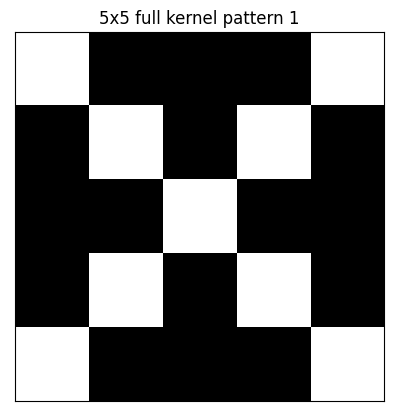
\includegraphics[width=0.49\textwidth]{../../code/serialization/kernels/5x5/full/5x5_kernel_full_1.png}
				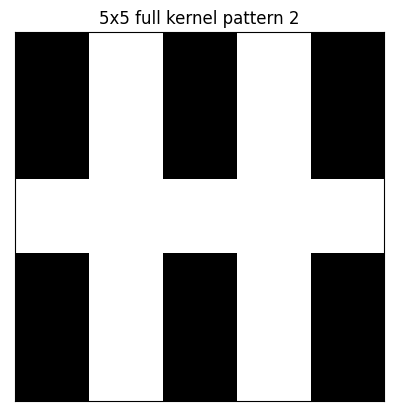
\includegraphics[width=0.49\textwidth]{../../code/serialization/kernels/5x5/full/5x5_kernel_full_2.png}
				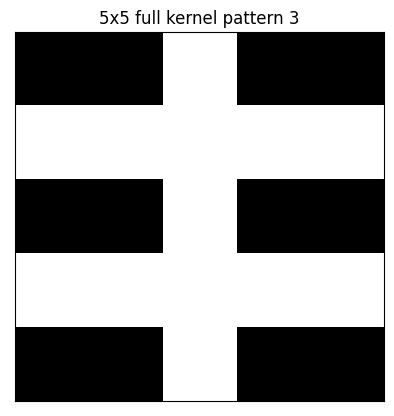
\includegraphics[width=0.49\textwidth]{../../code/serialization/kernels/5x5/full/5x5_kernel_full_3.png}
			\end{center}
			\caption{Non-zero elements of $\text{Null}(A_5)$}
		\end{figure}
	
		We can partition the squares of the $5 \times 5$ board to one of four regions based on which quiet patterns they are a part of.
		
		\begin{figure}[H]
		\begin{center}
			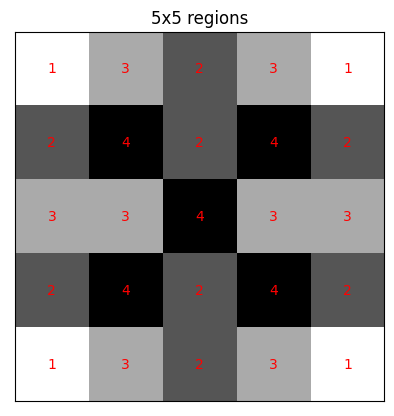
\includegraphics[width=0.49\textwidth]{../../code/serialization/regions/5x5_regions.png}
		\end{center}
		\end{figure}
	
		Region 1 is the intersection of quiet patterns 2 and 3; region 2 is the intersection of quiet patterns 1 and 2; region 3 is the intersection of quiet patterns 1 and 3;
		region 4 is in none of the quiet patterns.
		
		Let $M$ be the answer to the Min Moves Problem for a $5 \times 5$ board.
		Then there must exist some $5 \times 5$ board $\vec{b}$ that requires $M$ moves to solve optimally.
		Let $\vec{x}$ be a solution to $\vec{b}$ that uses $M$ moves.
		Let $A$ be the number of moves in $\vec{x}$ in region 1, $B$ in region 2, $C$ in region 3, and $D$ in region 4.
		Then the solution uses $M = A + B + C + D$ moves.
		
		If we apply quiet pattern 1, we obtain another solution to $\vec{b}$ that uses $A + (8 - B) + (8 - C) + D$ moves.
		Since we assumed $\vec{x}$ was already a minimal solution,
		\begin{equation*}
			A + B + C + D \leq A + (8 - B) + (8 - C) + D.
		\end{equation*}
		Rearranging,
		\begin{equation}\label{5x5_constr1}
			B + C \leq 8.
		\end{equation}
	
		If we apply quiet pattern 2, we obtain another solution to $\vec{b}$ that uses $(4 - A) + (8 - B) + C + D$ moves.
		Since we assumed $\vec{x}$ was already a minimal solution,
		\begin{equation*}
			A + B + C + D \leq (4 - A) + (8 - B) + C + D.
		\end{equation*}
		Rearranging,
		\begin{equation}\label{5x5_constr2}
			A + B \leq 6.
		\end{equation}
	
		If we apply quiet pattern 3, we obtain another solution to $\vec{b}$ that uses $(4 - A) + B + (8 - C) + D$ moves.
		Since we assumed $\vec{x}$ was already a minimal solution,
		\begin{equation*}
			A + B + C + D \leq (4 - A) + B + (8 - C) + D.
		\end{equation*}
		Rearranging,
		\begin{equation}\label{5x5_constr3}
			A + C \leq 6.
		\end{equation}
	
		None of \eqref{5x5_constr1}, \eqref{5x5_constr2}, or \eqref{5x5_constr3} affect $D$.
		Thus, $D$ is not constrained beyond the fact that region 4 contains five buttons.
		So, in any board that requires the maximum number of clicks to optimally solve, $D = 5$.
	
		Putting \eqref{5x5_constr1}, \eqref{5x5_constr2}, and \eqref{5x5_constr3} in matrix form,
		\begin{equation}\label{5x5_ilp}
			\begin{bmatrix}
				0 & 1 & 1 \\
				1 & 1 & 0 \\
				1 & 0 & 1
			\end{bmatrix}
			\begin{bmatrix}
				A \\
				B \\
				C
			\end{bmatrix}
			\leq
			\begin{bmatrix}
				8 \\
				6 \\
				6
			\end{bmatrix}.
		\end{equation}
		Thus, we need to solve this integer linear program (ILP), maximizing the $L^1$-norm $A + B + C$.
		
		Since all entries in the constraint matrix of \eqref{5x5_ilp} are non-negative, finding an integer solution where the constraints are tight (i.e. replace the $\leq$ in \eqref{5x5_ilp} with $=$) would be a solution to the ILP.
		
		Assuming the constraints are tight, we find that
		\begin{equation*}
			\begin{bmatrix}
				A \\
				B \\
				C
			\end{bmatrix}
			=
			\begin{bmatrix}
				2 \\
				4 \\
				4
			\end{bmatrix}
		\end{equation*}
		is the solution to the ILP.
		So, the solution to the Min Moves Problem for a $5 \times 5$ board is $M = A + B + C + D = 2 + 4 + 4 + 5 = 15$.
	\end{proof}

	\section{Inequality for Larger Boards}
	In \cite{anderson_feil}, Anderson and Feil provide the following alternative characterization of quiet patterns:
	
	\begin{theorem}[Anderson \& Feil]\label{alt-characterization-quiet-patterns}
		A vector $\vec{q} \in \Z^{n^2}_2$ is a quiet pattern of an $n \times n$ board if and only if every square on the $n \times n$ board contains an even number of on squares from $\vec{q}$ in its neighborhood (itself and its edge-adjacent squares).
	\end{theorem}
	That is, $\vec{q}$ is an even parity cover of the board.
	This is because the state of any light is uniquely determined by the parity of the number of times the lights in its neighborhood have been pressed. Using this alternative characterization, we can build quiet patterns for larger boards from smaller ones.
	
	\begin{theorem}\label{tiling-quiet-patterns}
		Let $d(n) = \dim(\text{Null}(A_n))$.
		Then for all $n,k \in \N$,
		\begin{equation*}
			d(nk - 1) \geq d(n-1).
		\end{equation*}
	\end{theorem}
	\begin{proof}
		Let $n,k \in \N$.
		Since $nk - 1 = k(n-1) + (k-1)$, an $(nk-1) \times (nk-1)$ board consists of a $k \times k$ grid of $(n-1) \times (n-1)$ boards, each separated by a horizontal or vertical strip of height or width 1.
	
		Let $\vec{q}$ be a quiet pattern for an $(n-1) \times (n-1)$ board.
		Let $\vec{Q}$ be $\vec{q}$ tiled $k$ times horizontally and vertically onto an $(nk-1) \times (nk-1)$ board, where each tile is a horizontal/vertical reflection of its horizontal/vertical neighboring tiles.
		
		\begin{figure}[H]
			\centering
%			\begin{tikzpicture}[scale=0.33]
%				\edef\M{3} % Width of each tile
%				\edef\K{5} % Number of tiles in each direction
%				\pgfmathparse{(\M+1)*\K - 1} % Size of large board
%				\edef\N{\pgfmathresult}
%				
%				\draw[black,thin] (0,0) grid (\N,\N);
%				
%				\foreach \i in {1,2,...,\K}{
%					\foreach \j in {1,2,...,\K}{
%						\pgfmathparse{(\i - 1) * (\M + 1)}
%						\edef\X{\pgfmathresult}
%						\pgfmathparse{(\j - 1) * (\M + 1)}
%						\edef\Y{\pgfmathresult}
%						
%						\draw[fill,gray,opacity=0.707] (\X, \Y) rectangle (\X + \M, \Y + \M);
%						%\node at (\X + \M/2, \Y + \M/2) {$Q$};
%					}
%				}
%			\end{tikzpicture}
			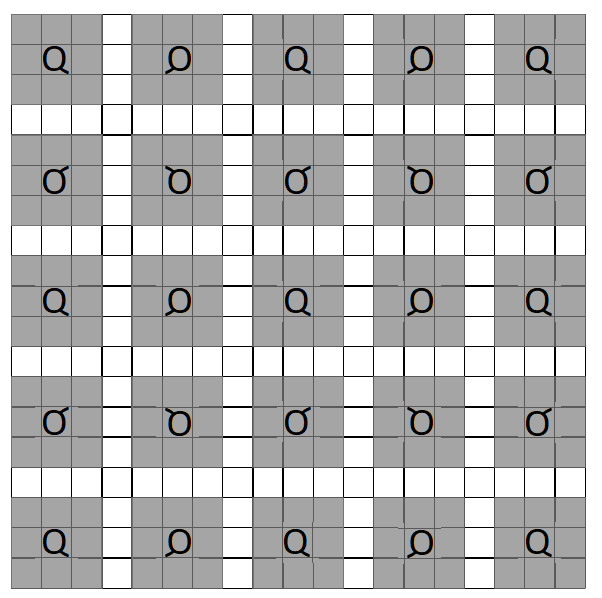
\includegraphics[width=0.5\textwidth]{tiling_q.png}
			\caption{Pattern $Q$ tiled 5 times.}	
		\end{figure}
	
		We will show that $\vec{Q}$ is a quiet pattern.
		Consider any square in the $(nk-1) \times (nk-1)$ board with $\vec{Q}$.
		If the square is one of the areas containing a reflection of $\vec{q}$, then the square's neighborhood contains an even number of 1's from $\vec{Q}$, since $\vec{q}$ is a quiet pattern.
		If the square is not one of these areas containing a reflection of $\vec{q}$, then the square itself is a 0 in $\vec{Q}$, and its neighborhood contains either zero or two squares that are reflections of $\vec{q}$.
		If there are zero such squares in the neighborhood, then the entire neighborhood contains zero 1's from $\vec{Q}$, which is even.
		If there are two such squares in the neighborhood, then the state of the two squares are the same because we reflected $\vec{q}$.
		Thus, the neighborhood contains either zero or two 1's from $\vec{Q}$, which in either case is even.
		Since the neighborhood of every square contains an even number of 1's from $\vec{Q}$, we see that $\vec{Q}$ is a quiet pattern.
		
		So, if we have an orthogonal basis for the quiet patterns for an $(n-1) \times (n-1)$ board, we can generate a mutually orthogonal set of quiet patterns on an $(nk-1) \times (nk-1)$ board, one element for each element of the basis. 
		Thus,
		\begin{equation*}
			d(nk-1) \geq d(n-1),
		\end{equation*}
		as desired.
	\end{proof}

	\section{Establishing an Upper Bound}
	Applying theorem \ref{tiling-quiet-patterns} for $n=6$, we get that for all $k \in \N$,
	\begin{equation*}
		d(6k - 1) \geq d(5) = 2.
	\end{equation*}
	For $(6k-1) \times (6k-1)$ boards, we know that we're tiling the $5 \times5 $ quiet patterns.
	For example, notice how the $17 \times 17$ quiet patterns are simply the $5 \times 5$ quiet patterns tiled $k=3$ times.
	
	\begin{figure}[H]
		\centering
		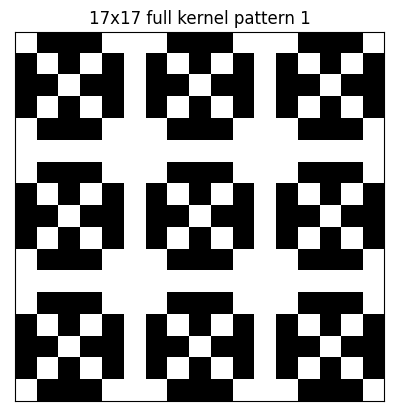
\includegraphics[width=0.49\textwidth]{../../code/serialization/kernels/17x17/full/17x17_kernel_full_1.png}
		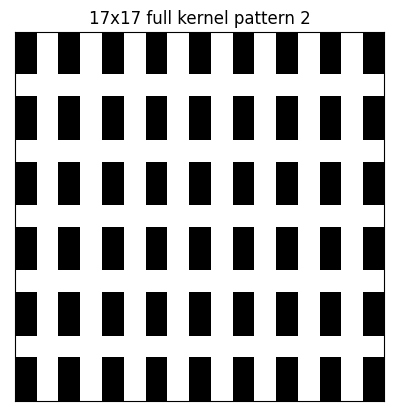
\includegraphics[width=0.49\textwidth]{../../code/serialization/kernels/17x17/full/17x17_kernel_full_2.png}
		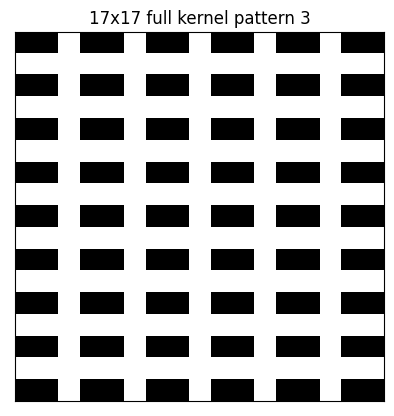
\includegraphics[width=0.49\textwidth]{../../code/serialization/kernels/17x17/full/17x17_kernel_full_3.png}
		\caption{Elements of $\text{Null}(A_{17})$}
	\end{figure}
	
	Thus, we can apply the same proof technique as in theorem \ref{min-moves-problem-5x5} to find an upper bound for the Min Moves Problem for such board sizes.
	We'll also know that if $d(6k - 1) = 2$, then this upper bound is exact, and we have solved the Min Moves Problem.
	
	\begin{theorem}\label{min-moves-problem-6k-1x6k-1}
		Let $k \in \N$.
		Then the solution to the Min Moves Problem for a $(6k - 1) \times (6k - 1)$ board is $26k^2 - 12k + 1$.
	\end{theorem}
	\begin{proof}
		Let $k \in \N$.
		Applying theorem \ref{tiling-quiet-patterns} with $n=6$, the non-zero quiet patterns of the $5 \times 5$ board will tile a $(6k - 1) \times (6k - 1)$ board.
		We can partition the squares of the board into four regions based on which quiet patterns the are a part of.
		Using the same numbering of quiet patterns as in theorem \ref{min-moves-problem-5x5}, region 1 is the intersection of quiet patterns 2 and 3; region 2 is the intersection of quiet patterns 1 and 2; region 3 is the intersection of quiet patterns 1 and 3; region 4 is none of the quiet patterns.
		Region 1 contains $4k^2$ squares, regions 2 and 3 both contain $8k^2$ squares, and region 4 contains the remaining $16k^2 - 12k + 1$ squares.
		
		Let $M$ be the answer to the Min Moves Problem for a $(6k-1) \times (6k-1)$ board where we only consider the quiet patterns tiled from a $5 \times 5$ board.
		There there may exist some $(6k-1) \times (6k-1)$ board $\vec{b}$ that uses $M$ moves to solve optimally.
		Let $\vec{x}$ be a solution to $\vec{b}$ that uses $M$ moves.
		Let $A$ be the number of moves in $\vec{x}$ in region 1, $B$ in region 2, $C$ in region 3, and $D$ in region 4.
		Then the solution uses $M = A + B + C + D$ moves.
		
		Applying the three quiet patterns and deriving the constraints, we find that $D$ is unconstrained by the quiet patterns and can thus be set to $16k^2 - 12k + 1$, while $A$, $B$, and $C$ are constrained by the following ILP:
		\begin{equation}
			\begin{bmatrix}
				0 & 1 & 1 \\
				1 & 1 & 0 \\
				1 & 0 & 1 
			\end{bmatrix}
			\begin{bmatrix}
				A \\
				B \\
				C
			\end{bmatrix}
			\leq
			\begin{bmatrix}
				8 \\
				6 \\
				6
			\end{bmatrix}k^2.
		\end{equation}
		This is the exact same set of constraints as in theorem \ref{min-moves-problem-5x5}, just with a factor of $k^2$.
		Thus,
		\begin{equation*}
			\begin{bmatrix}
				A \\
				B \\
				C
			\end{bmatrix}
			=
			\begin{bmatrix}
				2 \\
				4 \\
				4
			\end{bmatrix}k^2.
		\end{equation*}
		is the solution to the ILP.
		The solution to the Min Moves Problem for a $(6k-1) \times (6k-1)$ board is $M = A + B + C + D = 2k^2 + 4k^2 +  4k^2 + 16k^2 - 12k + 1 = 26k^2 - 12k + 1$, as desired.
	\end{proof}

	The reason this result is an upper bound and not tight as in theorem \ref{min-moves-problem-5x5} is that if there are other quiet patterns than the three we considered, there will be additional constraints.
	However, if we have indeed considered all quiet patterns then the bound is exact.

	\begin{corollary}\label{min-moves-6k-1-cor}
		This bound is exact for boards with nullity 2.
	\end{corollary}

	The $5 \times 5$, $17 \times 17$, $41 \times 41$, $53 \times 53$, $77 \times 77$, $113 \times 113$, $\dots$ boards are the boards of size $(6k-1) \times (6k-1)$ with nullity 2.
	Thus, applying corollary \ref{min-moves-6k-1-cor}, we find that the solutions to the Min Moves problem is 15, 199, 1191, 1999, 4239, 9159, $\dots$ respectively.
	
	\section{Conjectures}
	\begin{conjecture}
		If an $n \times n$ board has nullity 2, then $n \equiv -1 \mod 6$.
	\end{conjecture}
	That is, the quiet patterns of all nullity 2 boards are tilings of the $5 \times 5$ quiet patterns.
	If true, this would mean that we have solved the Min Moves Problem for all nullity 2 boards.

	\begin{conjecture}\label{ilp-conj}
		The proof technique of assuming our integer program can be solved with all constraints tight will only work for boards with nullity 2, none higher.
	\end{conjecture}
	That is, solving the ILP by assuming all constraints can be tightly satisfied does not work for boards with nullity greater than 2.
	
	\section{Future Work}
	We'd like future work to focus on solving boards with nullities greater than 2.
	For any sized board, we can apply the same technique as in theorems \ref{min-moves-problem-5x5} and \ref{min-moves-problem-6k-1x6k-1} of finding the solution to the Min Moves Problem as the solution to an ILP.
	However, as we state in conjecture \ref{ilp-conj}, it seems the ILP for larger nullities cannot be solved with all constraints tight.
	The $4 \times 4$ board with nullity 4 (nullities are always even) is the smallest with nullity greater than 2.
	We know via brute force that the answer to the Min Moves Problem in this case is 7.
	Perhaps if we better understood how to solve the ILP for the $4 \times 4$ board, we could generalize to larger boards.
	
	We'd also like future work to focus more on understanding the relationships between the nullities of different sized boards.
	The inequality derived in theorem \ref{tiling-quiet-patterns} is a good start to this, but there seem to be many other patterns to discover.
	For example, Sutner conjectures in \cite{Sutner1989} that $d(2n+1) = 2d(n) + \delta_n$, where $\delta_n \in \{0,2\}$, and $\delta_{2n+1} = \delta_n$.

	\newpage
	\bibliography{refs.bib}
	\bibliographystyle{amsplain}
\end{document}